%  LaTeX support: latex@mdpi.com 
%  In case you need support, please attach all files that are necessary for compiling as well as the log file, and specify the details of your LaTeX setup (which operating system and LaTeX version / tools you are using).

%=================================================================
%\documentclass[applsci,article,submit,moreauthors,pdftex]{template/mdpi} 
\documentclass[preprints,article,accept,moreauthors,pdftex]{template/mdpi}


%=================================================================
\firstpage{1} 
\makeatletter 
\setcounter{page}{\@firstpage} 
\makeatother
\pubvolume{xx}
\issuenum{1}
\articlenumber{5}
\pubyear{2019}
\copyrightyear{2019}
%\externaleditor{Academic Editor: name}
\history{Received: date; Accepted: date; Published: date}
%\updates{yes} % If there is an update available, un-comment this line

%% MDPI internal command: uncomment if new journal that already uses continuous page numbers 
%\continuouspages{yes}

%------------------------------------------------------------------
% The following line should be uncommented if the LaTeX file is uploaded to arXiv.org
%\pdfoutput=1

%=================================================================
% Add packages and commands here. The following packages are loaded in our class file: fontenc, calc, indentfirst, fancyhdr, graphicx, lastpage, ifthen, lineno, float, amsmath, setspace, enumitem, mathpazo, booktabs, titlesec, etoolbox, amsthm, hyphenat, natbib, hyperref, footmisc, geometry, caption, url, mdframed, tabto, soul, multirow, microtype, tikz

%=================================================================
%% Please use the following mathematics environments: Theorem, Lemma, Corollary, Proposition, Characterization, Property, Problem, Example, ExamplesandDefinitions, Hypothesis, Remark, Definition, Notation, Assumption
%% For proofs, please use the proof environment (the amsthm package is loaded by the MDPI class).

\graphicspath{{../img/}}

%=================================================================
% Full title of the paper (Capitalized)
\Title{Solar irradiance nowcasting using deep networks}

% Author Orchid ID: enter ID or remove command
\newcommand{\orcidauthorA}{0000-0000-000-000X} % Add \orcidA{} behind the author's name
%\newcommand{\orcidauthorB}{0000-0000-000-000X} % Add \orcidB{} behind the author's name

% Authors, for the paper (add full first names)
\Author{Firstname Lastname $^{1,\dagger,\ddagger}$\orcidA{}, Firstname Lastname $^{1,\ddagger}$ and Firstname Lastname $^{2,}$*}

% Authors, for metadata in PDF
\AuthorNames{Firstname Lastname, Firstname Lastname and Firstname Lastname}

% Affiliations / Addresses (Add [1] after \address if there is only one affiliation.)
\address{%
$^{1}$ \quad Affiliation 1; e-mail@e-mail.com\\
$^{2}$ \quad Affiliation 2; e-mail@e-mail.com}

% Contact information of the corresponding author
\corres{Correspondence: e-mail@e-mail.com; Tel.: (optional; include country code; if there are multiple corresponding authors, add author initials) +xx-xxxx-xxx-xxxx (F.L.)}

% Current address and/or shared authorship
\firstnote{Current address: Affiliation 3} 
\secondnote{These authors contributed equally to this work.}
% The commands \thirdnote{} till \eighthnote{} are available for further notes

%\simplesumm{} % Simple summary

%\conference{} % An extended version of a conference paper

% Abstract (Do not insert blank lines, i.e. \\) 
\abstract{Accurate solar irradiance nowcasting using deep neural networks. Robust to missing values in sensors. Study of influence of the wind in the prediction. Interpolation of missing values using Gaussian process regression. A strategy to place new sensors in order to improve accuracy on target sensors.}

% Keywords
\keyword{Solar Irradiance; Nowcasting; Deep Neural Networks; Gaussian Processes. }

% The fields PACS, MSC, and JEL may be left empty or commented out if not applicable
%\PACS{J0101}
%\MSC{}
%\JEL{}

%%%%%%%%%%%%%%%%%%%%%%%%%%%%%%%%%%%%%%%%%%
% Only for the journal Diversity
%\LSID{\url{http://}}

%%%%%%%%%%%%%%%%%%%%%%%%%%%%%%%%%%%%%%%%%%
% Only for the journal Applied Sciences:
%\featuredapplication{Authors are encouraged to provide a concise description of the specific application or a potential application of the work. This section is not mandatory.}
%%%%%%%%%%%%%%%%%%%%%%%%%%%%%%%%%%%%%%%%%%

%%%%%%%%%%%%%%%%%%%%%%%%%%%%%%%%%%%%%%%%%%
% Only for the journal Data:
%\dataset{DOI number or link to the deposited data set in cases where the data set is published or set to be published separately. If the data set is submitted and will be published as a supplement to this paper in the journal Data, this field will be filled by the editors of the journal. In this case, please make sure to submit the data set as a supplement when entering your manuscript into our manuscript editorial system.}

%\datasetlicense{license under which the data set is made available (CC0, CC-BY, CC-BY-SA, CC-BY-NC, etc.)}

%%%%%%%%%%%%%%%%%%%%%%%%%%%%%%%%%%%%%%%%%%
% Only for the journal Toxins
%\keycontribution{The breakthroughs or highlights of the manuscript. Authors can write one or two sentences to describe the most important part of the paper.}

%\setcounter{secnumdepth}{4}
%%%%%%%%%%%%%%%%%%%%%%%%%%%%%%%%%%%%%%%%%%
\begin{document}
%%%%%%%%%%%%%%%%%%%%%%%%%%%%%%%%%%%%%%%%%%

\section{TODO}
\begin{itemize}
    \item Introduction of problem.
    \item Literature review.
    \item Data preprocessing in Section \ref{sec:prep}.
    \item Description of models in Section \ref{sec:models}.
    \item Write results of different models in Section \ref{sec:results}.
    \item Compare results with other papers?
    \item Repeat models using wind data. Are we improving?
    \item Write nice story about wind influence in Section \ref{subsec:wind}.
    \item Include robustness study in Section \ref{subsec:robust}.
    \item Think and write framework for sensor positioning in Section \ref{sec:positioning}.
    \item Write conclusions in Section \ref{sec:conclusions}.

\end{itemize}

%%%%%%%%%%%%%%%%%%%%%%%%%%%%%%%%%%%%%%%%%%%%
\section{To Decide}
\begin{itemize}
    \item Remove Robustness.
    \item Join related work and introduction in a compact section.

\end{itemize}
%%%%%%%%%%%%%%%%%%%%%%%%%%%%%%%%%%%%%%%%%%
\section{Introduction}\label{sec:intro}

Solar irradiance estimation has critical applications in the forecasting of energy generation from solar power plants, the heating and cooling loads of buildings, and in weather forecasting and climate modeling. Thus, it is of vital importance to develop systems that make accurate predictions to increase the performance of posterior decision making systems. On the other hand, the volume of generated data from sensor measurements has quickly exploded in the past years, making the development of efficient and scalable algorithms that require little human tuning a requirement.

\subsection{Related work}

Previous approaches to the solar irradiance nowcasting problem has been based on...


In this work, we propose the design and application of deep neural networks for solar irradiance nowcasting. We test empirically the accuracy of the proposed approach using the OAHU dataset. We observe that there is a strong spatial pattern in the accuracy of the predictions which is clearly related with the wind direction. In light of these results, we perform a thorough analysisis of the influence of the wind in solar irradiance nowcasting. This analysis suggest a strategy to place new sensors in order to improve accuracy on different targets that we present in Section \ref{sec:positioning}.


What problems will be addressed in the paper?
\begin{itemize}
    \item Propose a framework to do short term forecasting of solar irradiance which is robust to missing values in sensors. 
    \item Discuss why is this problem important.
    \item Study robustness.
    \item Study influence of wind direction.
    \item Propose a strategy to place new sensors in order to improve accuracy on target sensors.
\end{itemize}


%%%%%%%%%%%%%%%%%%%%%%%%%%%%%%%%%%%%%%%%%%
\section{Data preprocessing}\label{sec:prep}

\begin{figure}
\centering
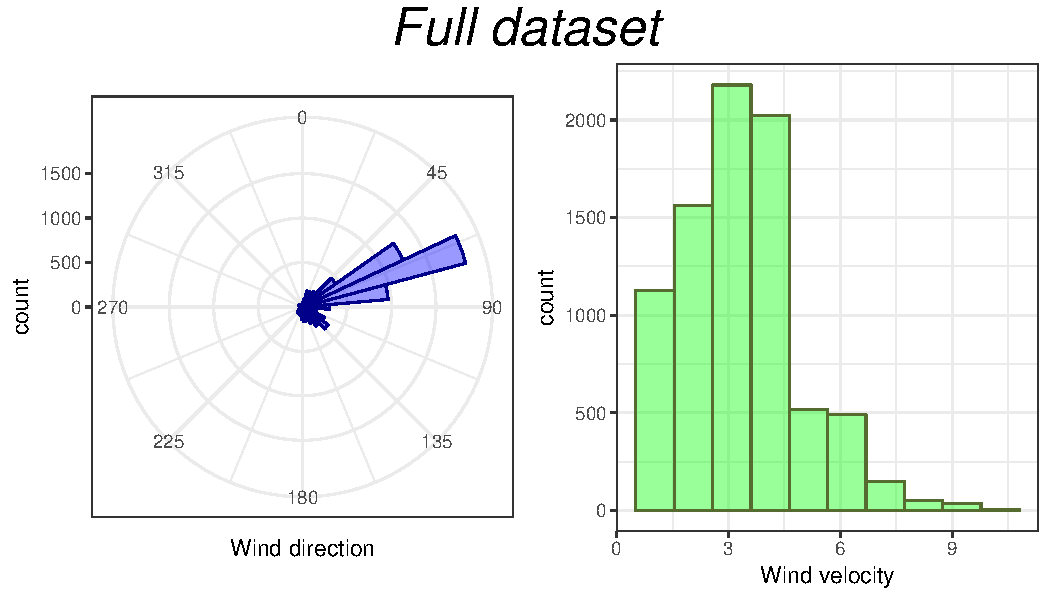
\includegraphics[width=\textwidth]{Clear_dataset.pdf}
\caption{Caption here}
\end{figure}


%%%%%%%%%%%%%%%%%%%%%%%%%%%%%%%%%%%%%%%%%%
%%%%%%%%%%%%%%%%%%%%%%%%%%%%%%%%%%%%%%%%%%
\section{Deep Networks in solar irradiance nowcasting}\label{sec:models}

In this Section we describe several architectures developed and tested for the solar irradiance nowcasting task. All models from this Section are based on deep artificial neural networks \cite{Goodfellow-et-al-2016}, since they offer greater flexibility compared to shallower models for data in which complex, non-linear interactions may arise. 

The models were implemented in Python, using the \texttt{tensorflow} \cite{abadi2016tensorflow} and \texttt{keras} \cite{chollet2015keras} frameworks for deep learning. With the aim of enabling reproducible research, the code for running the experiments is located at \url{https://github.com/albertotb/solar}.

\subsection{Convolutional architectures}

Convolutional neural networks \cite{krizhevsky2012imagenet} have recently gained vast interest as they have become the \emph{state of the art} model for image and signal processing tasks \cite{ji20123d, karpathy2014large, abdel2014convolutional}. By replacing a dense linear projection with a convolution operation, these networks exploit the data invariances to location and scaling and greatly reduce the number of parameters.

In the following subsections we describe several alternatives developed to arrange the sensor data in a more profitable way for the convolutional models.

\subsubsection{1D convolutional}

Stemming from the hypothesis that the forecast of any given sensor might be improved using the information of nearby sensors, a first sensor arrangement can be obtained by sorting the sensors by their geographical longitude, that is, $ x_{\sigma_{long}(i),t} \in \mathbb{R}$ will denote the solar irradiance measured at time-step $t$ and sensor $i \in \lbrace 1, \ldots, 17 \rbrace$, where $\sigma_{long}$ is a permutation that sorts the indices in non-decreasing longitude coordinate (CHECK).

Then, we applied a series of one-dimensional convolutional layers, which have shown superb performance in diverse tasks such as sentence classification \cite{kim2014convolutional}.

Distinguish between locally-connected and 1d convolutional...

Residual connection to upper-bound the persistence model...

\subsubsection{2D convolutional}

Since we only have a discrete set of measurements over a spatial region, we propose to use Gaussian process regression  \cite{rasmussen2003gaussian} (a.k.a. \emph{kriging}) to spatially interpolate between sensor measurements and obtain a bidimensional irradiation map.

Then, we use a standard 2D convolutional layer...



\subsection{Recurrent architectures}

In order to avoid a fixed window size, we explore the applicability of recurrent layers, in particular the \emph{long-short term memory} (LSTM) network \cite{gers1999learning}.

Mention the convolutional-recurrent architectures which have found great success in tasks such as scene labelling \cite{pinheiro2014recurrent} and text classification \cite{lai2015recurrent}.

\subsection{Optimization}

In this Section we describe the training procedure. All models were optimized using the backpropagation algorithm \cite{Rumelhart:1986:LIR:104279.104293} through the automatic differentiation library \texttt{tensorflow}. The chosen optimizer was Adam, which is a popular modification of the standard stochastic gradient descent algorithm \cite{kingma2014adam}.

Regularization, hyperparameters and cross-validations...

%%%%%%%%%%%%%%%%%%%%%%%%%%%%%%%%%%%%%%%%%%

%%%%%%%%%%%%%%%%%%%%%%%%%%%%%%%%%%%%%%%%%%
\section{Experimental results}\label{sec:results}

Table \ref{tbl:preds} reports the results over the test dataset.

\begin{table}[!ht]
\centering
\caption{Prediction metrics over the held-out period.}\label{tbl:preds}
\begin{tabular}{lcc}
\cline{1-3}
   & \textbf{MAE}                             & \textbf{Metric 2}   \\ 
 \cline{1-3}
    Model 1          & $0.270$ &  $0.239$ \\
    Model 2          & $2.537$ &  $2.401$ \\
    Etc & $15.247$ & $13.461$\\
 \cline{1-3}
\end{tabular}
\end{table}



\subsection{Wind influence}\label{subsec:wind}



\subsection{Robustness}\label{subsec:robust}

%%%%%%%%%%%%%%%%%%%%%%%%%%%%%%%%%%%%%%%%%%

%%%%%%%%%%%%%%%%%%%%%%%%%%%%%%%%%%%%%%%%%%
\section{An efficient sensor positioning approach}\label{sec:positioning}
Given the influence of wind direction in solar irradiance nowcasting, we propose a efficient approach to place sensors in order to improve accuracy on target sensors...

(in what sense it is efficient!?)
%%%%%%%%%%%%%%%%%%%%%%%%%%%%%%%%%%%%%%%%%%

%%%%%%%%%%%%%%%%%%%%%%%%%%%%%%%%%%%%%%%%%%
\section{Conclusions}\label{sec:conclusions}

In this work we have found the following take-away points:

\begin{itemize}
    \item Leveraging the expressive power of deep, non-linear models helps in solar irradiance forecasting.
    \item Data arrangements specially tailored to convolutional models (1D and Gaussian process interpolation).
    \item Helps auxiliary tasks such as robustness and sensor placement.
\end{itemize}

Several lines of further work are possible:
\begin{itemize}
    \item Design of energy-efficient network architectures, such as the MobileNet model \cite{howard2017mobilenets}, so they can be deployed \emph{in situ} over low-cost hardware.
    \item Application of Bayesian models for forecasting a full predictive distribution, not only a point estimate.
\end{itemize}


%%%%%%%%%%%%%%%%%%%%%%%%%%%%%%%%%%%%%%%%%%
\vspace{6pt} 
\newpage
%%%%%%%%%%%%%%%%%%%%%%%%%%%%%%%%%%%%%%%%%%
%% optional
%\supplementary{The following are available online at \linksupplementary{s1}, Figure S1: title, Table S1: title, Video S1: title.}

% Only for the journal Methods and Protocols:
% If you wish to submit a video article, please do so with any other supplementary material.
% \supplementary{The following are available at \linksupplementary{s1}, Figure S1: title, Table S1: title, Video S1: title. A supporting video article is available at doi: link.}

%%%%%%%%%%%%%%%%%%%%%%%%%%%%%%%%%%%%%%%%%%
\authorcontributions{For research articles with several authors, a short paragraph specifying their individual contributions must be provided. The following statements should be used ``conceptualization, X.X. and Y.Y.; methodology, X.X.; software, X.X.; validation, X.X., Y.Y. and Z.Z.; formal analysis, X.X.; investigation, X.X.; resources, X.X.; data curation, X.X.; writing--original draft preparation, X.X.; writing--review and editing, X.X.; visualization, X.X.; supervision, X.X.; project administration, X.X.; funding acquisition, Y.Y.'', please turn to the  \href{http://img.mdpi.org/data/contributor-role-instruction.pdf}{CRediT taxonomy} for the term explanation. Authorship must be limited to those who have contributed substantially to the work reported.}

%%%%%%%%%%%%%%%%%%%%%%%%%%%%%%%%%%%%%%%%%%
\funding{This research received no external funding.}

%%%%%%%%%%%%%%%%%%%%%%%%%%%%%%%%%%%%%%%%%%
\acknowledgments{The authors acknowledge support from ...}

%%%%%%%%%%%%%%%%%%%%%%%%%%%%%%%%%%%%%%%%%%
\conflictsofinterest{The authors declare no conflict of interest.} 

%%%%%%%%%%%%%%%%%%%%%%%%%%%%%%%%%%%%%%%%%%
%% optional
\abbreviations{The following abbreviations are used in this manuscript:\\

\noindent 
\begin{tabular}{@{}ll}
MDPI & Multidisciplinary Digital Publishing Institute\\
LSTM & long short term memory \\
MAE & mean absolute error \\
\end{tabular}}

%%%%%%%%%%%%%%%%%%%%%%%%%%%%%%%%%%%%%%%%%%
%% optional
\appendixtitles{no} %Leave argument "no" if all appendix headings stay EMPTY (then no dot is printed after "Appendix A"). If the appendix sections contain a heading then change the argument to "yes".
\appendix
\section{}
\unskip
\subsection{}
Something

%%%%%%%%%%%%%%%%%%%%%%%%%%%%%%%%%%%%%%%%%%
\reftitle{References}

% Please provide either the correct journal abbreviation (e.g. according to the “List of Title Word Abbreviations” http://www.issn.org/services/online-services/access-to-the-ltwa/) or the full name of the journal.
% Citations and References in Supplementary files are permitted provided that they also appear in the reference list here. 

%=====================================
% References, variant A: external bibliography
%=====================================
%\externalbibliography{yes}
\bibliography{references}

%=====================================
% References, variant B: internal bibliography
%=====================================
%\begin{thebibliography}{999}
% Reference 1
%\bibitem[Author1(year)]{ref-journal}
%Author1, T. The title of the cited article. {\em Journal Abbreviation} {\bf 2008}, {\em 10}, 142--149.
%\end{thebibliography}

% The following MDPI journals use author-date citation: Arts, Econometrics, Economies, Genealogy, Humanities, IJFS, JRFM, Laws, Religions, Risks, Social Sciences. For those journals, please follow the formatting guidelines on http://www.mdpi.com/authors/references
% To cite two works by the same author: \citeauthor{ref-journal-1a} (\citeyear{ref-journal-1a}, \citeyear{ref-journal-1b}). This produces: Whittaker (1967, 1975)
% To cite two works by the same author with specific pages: \citeauthor{ref-journal-3a} (\citeyear{ref-journal-3a}, p. 328; \citeyear{ref-journal-3b}, p.475). This produces: Wong (1999, p. 328; 2000, p. 475)


%%%%%%%%%%%%%%%%%%%%%%%%%%%%%%%%%%%%%%%%%%
%% optional
%\sampleavailability{Samples of the compounds ...... are available from the authors.}

%% for journal Sci
%\reviewreports{\\
%Reviewer 1 comments and authors’ response\\
%Reviewer 2 comments and authors’ response\\
%Reviewer 3 comments and authors’ response
%}

%%%%%%%%%%%%%%%%%%%%%%%%%%%%%%%%%%%%%%%%%%
\end{document}

